\documentclass{article}

\usepackage{amsmath}
\usepackage{graphicx}
\usepackage[italian]{babel}
\usepackage{animate}
\usepackage{verbatim}

\title{Relazione per il Primo Progetto di Algoritmi e Strutture Dati e Laboratorio}
\date{16-07-2020}
\author{Alessandro Zanatta \\ 143154 \\ zanatta.alessandro@spes.uniud.it\\ \and Christian Abbondo \\ 144033 \\ abbondo.christian@spes.uniud.it\\ \\}

\begin{document}

	% Generate first page with no page numbers
	\pagenumbering{gobble}
	\maketitle
	\newpage
	
	
	% Generate table of contents (entries correspond to sections, subsections, ...)
	\pagenumbering{arabic}
	\tableofcontents	
	\newpage
	
	\section{Introduzione}
	La seguente relazione si propone di analizzare i tempi di esecuzione di tre algoritmi utilizzati per trovare il $k$-esimo elemento più piccolo di un array: 
	\begin{itemize}
		\item QuickSelect
		\item HeapSelect
		\item MedianSelect
	\end{itemize}
	 
	Il linguaggio scelto e utilizzato per implementare le strutture dati e gli algoritmi, nonchè per il calcolo dei tempi di esecuzione, è C, in quanto è indubbiamente uno dei linguaggi più efficienti e veloci, al costo di una maggiore complessità del codice. \\ In questo modo i tempi di esecuzione ottenuti sono liberi da controlli aggiuntivi che altri linguaggio di programmazione effettuano.
	\newpage
	
	
	\section{Aspettative teoriche}
	In questa sezione si discuteranno le aspettative teoriche relative ai tempi di esecuzione degli algoritmi in questione.
	\\
	Ricordiamo, innanzitutto, il costo asintotico degli algoritmi in analisi:
	
	
	\begin{itemize}
		\item QuickSort $\rightarrow$ $O\left(n^{2}\right)$, nel caso peggiore, $O\left(n\right)$, nel caso medio
		\item HeapSelect $\rightarrow$ $O(n + k\log{k})$ sia nel caso peggiore che in quello medio
		\item MedianSelect $\rightarrow$ $\Theta(n)$ in qualsiasi caso
	\end{itemize}
	
	\paragraph{QuickSelect}
	Ci si aspetta che l'algoritmo, al verificarsi del caso peggiore, sia il meno efficiente fra i tre, dato il suo costo asintotico maggiore. Nel caso medio, tuttavia, questo algoritmo potrebbe risultare più efficiente di HeapSelect e di MedianSelect.
	
	\paragraph{HeapSelect}
	\label{section:theory}
	L'algoritmo, in quanto dipendente da $k$, avrà costo differente in base al parametro $k$.
	In particolare, il costo sarà $\Theta\left(n\right)$ nel caso in cui $k\in\Theta(1)$ e di $O\left(n + k\cdot\log{k}\right)$ per $k\in\Theta\left(n\right)$. L'algoritmo sarà particolarmente efficiente, quindi, per $k$ costante, mentre tenderà a essere piuttosto inefficiente per $k\approx n$.\footnote{Dato che si è scelto di implementare l'algoritmo HeapSelect utilizzando opportunamente minheaps o maxheaps (in base al parametro $k$), il costo dell'algoritmo sarà differente. Il costo effettivo sarà discusso nelle prossime pagine.} 
	
	\paragraph{MedianSelect}
	Questo algoritmo, considerato che è una versione ottimizzata di QuickSelect	e che il costo asintotico è, nel caso peggiore, minore di quello di QuickSelect, dovrebbe risultare più efficiente. In particolare, per $k\approx n$, MedianSelect dovrebbe essere più efficiente sia di QuickSelect che di HeapSelect\footnote{Come già riportato, per l'implementazione scelta il costo sarà diverso e verrà discusso nella prossima sezione dell'elaborato.}.
	
	\newpage
	
	\section{Note implementative}
	\label{section:impl_notes}
	Si discutono ora alcune scelte implementative effettuate.
	
	\paragraph{HeapSelect}
	L'algoritmo HeapSelect è stato implementato tenendo conto del parametro $k$. In particolare, l'algoritmo utilizzerà delle minheap se $k\leq \frac{n}{2}$, altrimenti userà delle maxheap. In questo modo, vengono effettuati al più $\frac{n}{2}$ estrazioni dalla seconda heap. \\ Considerata l'implementazione, è necessario riformulare le ipotesi enunciate finora. \\ Il costo dell'algoritmo è ora definito come:
	
	\[
		T\left(n\right) =
			\begin{cases}
				O\left(n + k\log{k}\right)  & \text{se $1\leq k \leq \frac{n}{2}$,} \\
				O\left(n + \left(n-k\right)\cdot\log{\left(n-k\right)}\right) & \text{se $\frac{n}{2} < k \leq n$} 
			\end{cases}
			\tag{1}
			\label{eq:heap}
	\]
	
	Risulta quindi ovvio che il costo massimo dell'algoritmo si otterrà per $k\approx \frac{n}{2} \in \Theta\left(n\right)$. Sebbene asintoticamente l'algoritmo pare avere un costo identico, è molto probabile che i tempi di esecuzione sperimentali rispecchieranno questa implementazione.
	
	\paragraph{MedianSelect} 
	Si è scelto di implementare l'algoritmo MedianSelect in place. Per farlo, si è semplicemente effettuato uno scambio della mediana calcolata sul singolo blocchetto di 5 elementi in una delle prime $\lceil\frac{n}{5}\rceil$ posizioni del vettore considerate dalla chiamata ricorsiva corrente. Si è inoltre trasformata la ricerca ricorsiva di un buon perno in iterativa. In questo modo si evita l'utilizzo dello spazio aggiutivo richiesto sullo stack dal frame di attivazione necessario per la chiamata ricorsiva stessa.
	
	\paragraph{Generazione di numeri pseudo-casuali}
	Dato che la funzione $\text{rand()}$ di C è piuttosto lenta e tende a fornire gli stessi interi dopo un numero relativamente piccolo di iterazioni, si utilizzerà una implementazione dell'algoritmo Mersenne Twister.
	
	\newpage
	\section{Calcolo del tempi di esecuzione}	
	Si riportano di seguito alcune	considerazioni riguardo il calcolo dei tempi effettuato nell'elaborato.
	
	\paragraph{Risoluzione}
	Si è scelto di utilizzare il clock offerto dalla funzione $\text{clock\_gettime}$. Il primo parametro della funzione indica il tipo di clock, mentre il secondo parametro è un puntatore ad una struct contentente il tempo all'istante della chiamata a funzione. Il tipo di clock utilizzato ($\text{CLOCK\_MONOTONIC\_RAW}$) è, come suggerito dal nome stesso, di tipo monotonico. \\ Per ottenere una misurazione della risoluzione migliore si è utilizzata la risoluzione mediana, calcolata su un campione di 10000 elementi.
	
	\paragraph{Scomputazione dell'inizializzazione}
	Al fine di scomputare correttamente dai tempi di esecuzione degli algoritmi il tempo di inizializzazione di un vettore casuale, si è utilizzata una funzione apposita che calcola il tempo mediano di tale operazione. Al fine di ottenere un errore relativo minore di $0.5\%$ si è ripetuta l'inizializzazione sufficienti volte affinché la seguente equazione fosse soddisfatta:
	
	\[
		\text{diff}\left(end, start\right) > resolution \cdot \left(1+\frac{1}{0.005}\right)  
	\]
	
	dove $\text{diff}$ indica l'intervallo temporale trascorso fra $start$ e $end$ e $resolution$ è la risoluzione del clock utilizzato. \\ Questo procedimento è stato poi iterato un certo numero di volte e dal campione di dati ottenuto si è estratta la mediana.
	
	\paragraph{Tempo di esecuzione degli algoritmi}
	Per ottenere misurazioni con errore relativo minore di $0.5\%$ si è operato nel seguente modo:
	
	\begin{itemize}
		\item Calcolo del tempo di inizializzazione di un vettore di data lunghezza secondo la procedura descritta nel paragrafo precedente
		\item Inizializzazione del vettore casuale e calcolo del tempo di esecuzione dell'algoritmo scelto. Si itera questo passaggio finché non è soddisfatta la seguente equazione:
		
			\[
				\text{diff}\left(end, start\right) > initialization + resolution \cdot \left(1+\frac{1}{0.005}\right)  
			\]
			
			dove $initialization$ è il tempo calcolato al primo punto.
	\end{itemize}
	
	% the paragraph under this does not fit in the current page :/
	\newpage
	
	\paragraph{Errore relativo massimo totale}
	Calcolando i tempi nei modi indicati negli ultimi due paragrafi si è ottenuto un errore relativo complessivo $\leq1\%$. L'errore relativo totale è, infatti, dato dalla somma degli errori. Essendoci quindi due misurazioni affette da errore\footnote{La prima è quella relativa al calcolo del tempo di inizializzazione, la seconda è quella relativa al tempo di esecuzione dell'algoritmo.}, entrambe con errore relativo pari o minore a $0.5\%$, l'errore relativo massimo totale è effettivamente dell'$1\%$.
	
	\paragraph{Problematiche riscontrate}
	Durante le prime misurazioni, si era notata una deviazione standard piuttosto elevata, indice di una grande variabilità nelle misurazioni ottenute. Al fine di ottenere delle misurazioni migliori, cioè meno sensibili ad outliers e rumore, si è scelto di utilizzare, al posto della media, la mediana dei tempi di esecuzione e, al posto della deviazione standard, la deviazione mediana assoluta, definita come $\textrm{MAD}=\textrm{median}\left(\mathopen|X_{i}-\textrm{median}\left(X\right)\mathclose|\right)$. Questi indici, in quanto indici di posizione, sono più robusti della media e della deviazione standard e hanno permesso di ottenere dei tempi sperimentali più accurati e minormente affetti da errori casuali.
	
	\newpage	
	\section{Analisi degli algoritmi}
	Per la valutazione dei tre diversi algoritmi sono stati utilizzati diversi criteri e sono state considerate diverse casistiche ritenute interessanti. In particolare, ci si soffermerà sui seguenti casi:
	
	\begin{itemize}
		\item Lunghezza $n$ dell'array variabile e $k=\frac{n}{3}$
		\item Lunghezza $n=75000$ e $k$ variabile in $[0,n-1]$
		\item Lunghezza $n$ variabile e $k=1$
	\end{itemize}
	
	\newpage
	
	\subsection{Lunghezza $n$ dell'array variabile e $k=\frac{n}{3}$}
	\label{subsection:nvar_k_n3}
	Iniziamo dall'analisi del grafico di un caso generale.
	
	\begin{figure}[h!]
		\centering
  		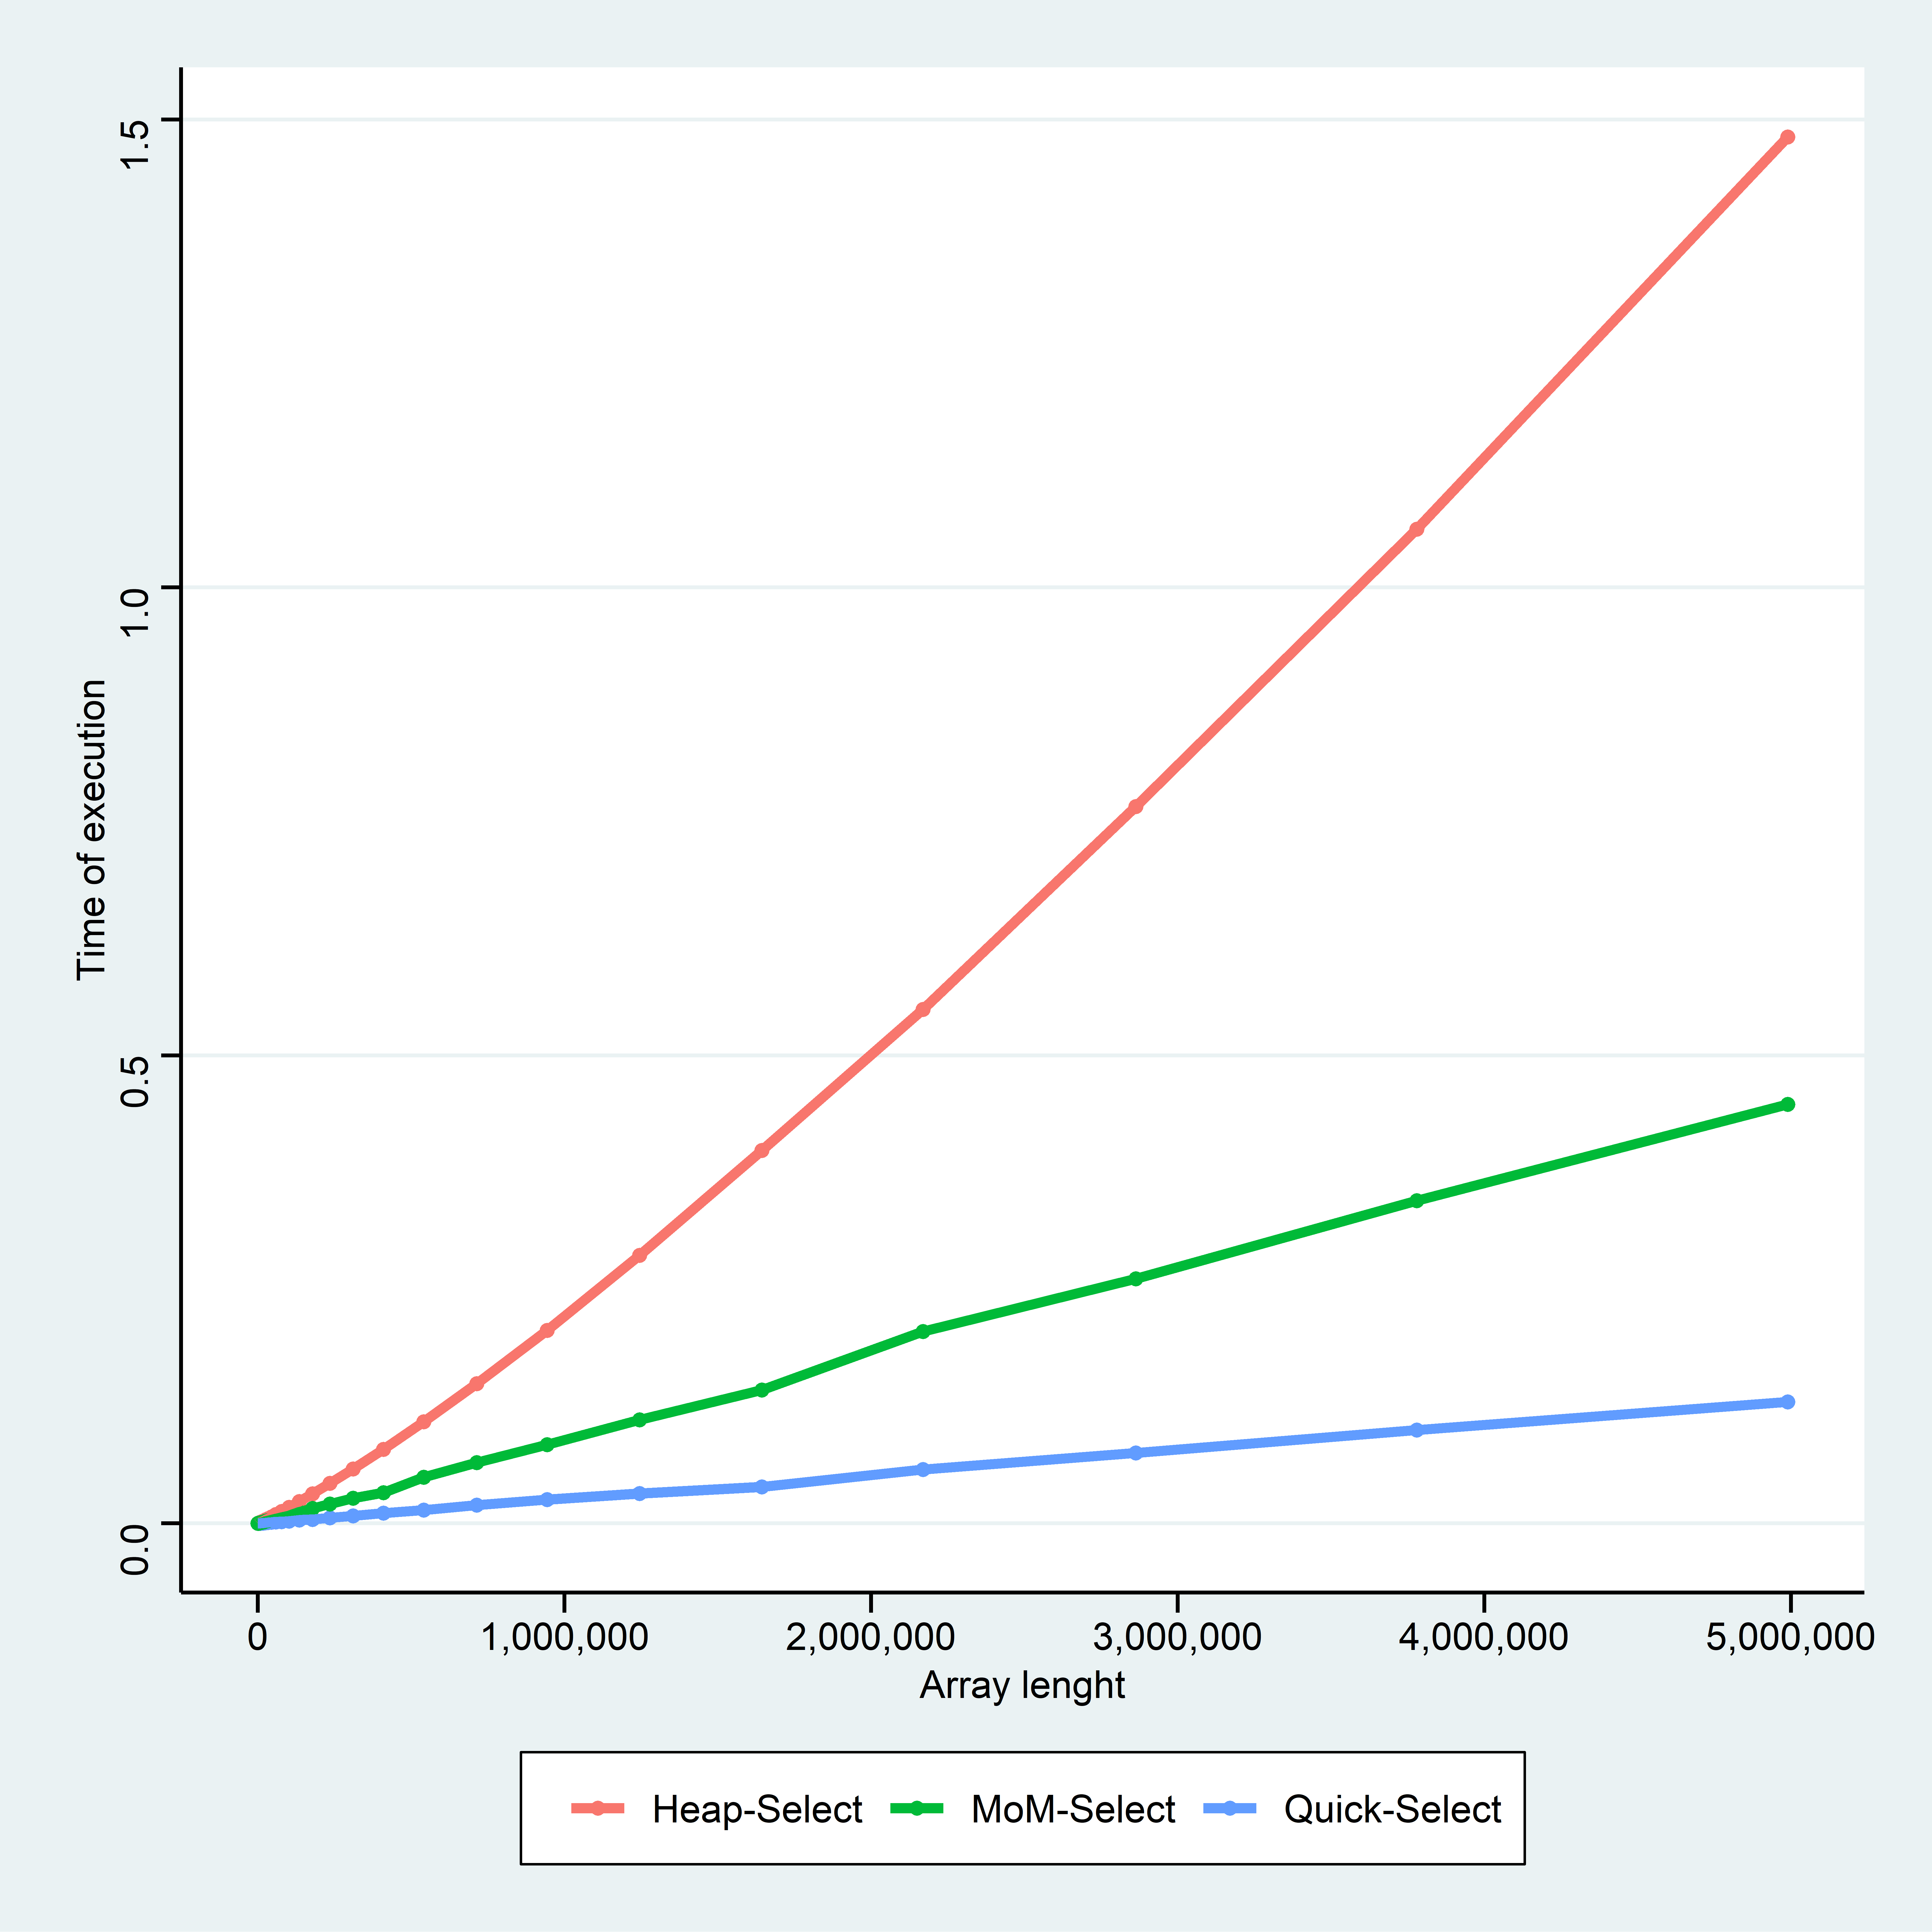
\includegraphics[width=0.9	\columnwidth]{images/All_Basic_Times.png}
  		\caption{Tempo di esecuzione a confronto per $n$ variabile e $k=\frac{n}{3}$}
  		\label{fig:graph1}
	\end{figure}	
	
	I risultati sperimentali ottenuti sembrano, in primo luogo, contraddirre le ipotesi formulate. Una analisi più approfondita, tuttavia, rivela che i risultati ottenuti sono sensati, nonchè interessanti. 
	\\\\
	Analizziamo innanzitutto il comportamento apparentemente anomalo di QuickSelect e MedianSelect.
	\\
	Le ipotesi teoriche non trovano riscontro nel grafico dei tempi ottenuto in quanto ci si aspetterebbe una maggiore efficienza di MedianSelect rispetto a QuickSelect. Tuttavia è da considerare un aspetto caratterizzante dell'algoritmo QuickSelect: il caso peggiore si verifica quando il vettore di input è fortemente ordinato (a causa della cattiva scelta del perno utilizzato per partizionare il vettore stesso). Dato che il vettore di input è stato generato il maniera pseudo-casuale, risulta chiaro che questo caso peggiore sia praticamente irrealizzabile. 
	\\
	Pertanto, è logico che l'algoritmo QuickSelect risulti, in pratica, più efficiente rispetto a MedianSelect, in quanto il primo sceglierà comunque, mediamente, dei buoni perni (a causa della casualità dell'input), svolgendo una quantità di lavoro minore rispetto alla sua versione ottimizzata. Entrambi gli algoritmi hanno quindi tempo di esecuzione lineare per vettori generati casualmente. 
	\\ 
	A comprovare questo fatto si ha il grafico sottostante, che dimostra come l'algoritmo QuickSelect sia effettivamente meno efficiente (e, in particolare, impieghi un tempo più che lineare) se il vettore di input è fortemente ordinato.
	
	\begin{figure}[h!]		
		\centering
  		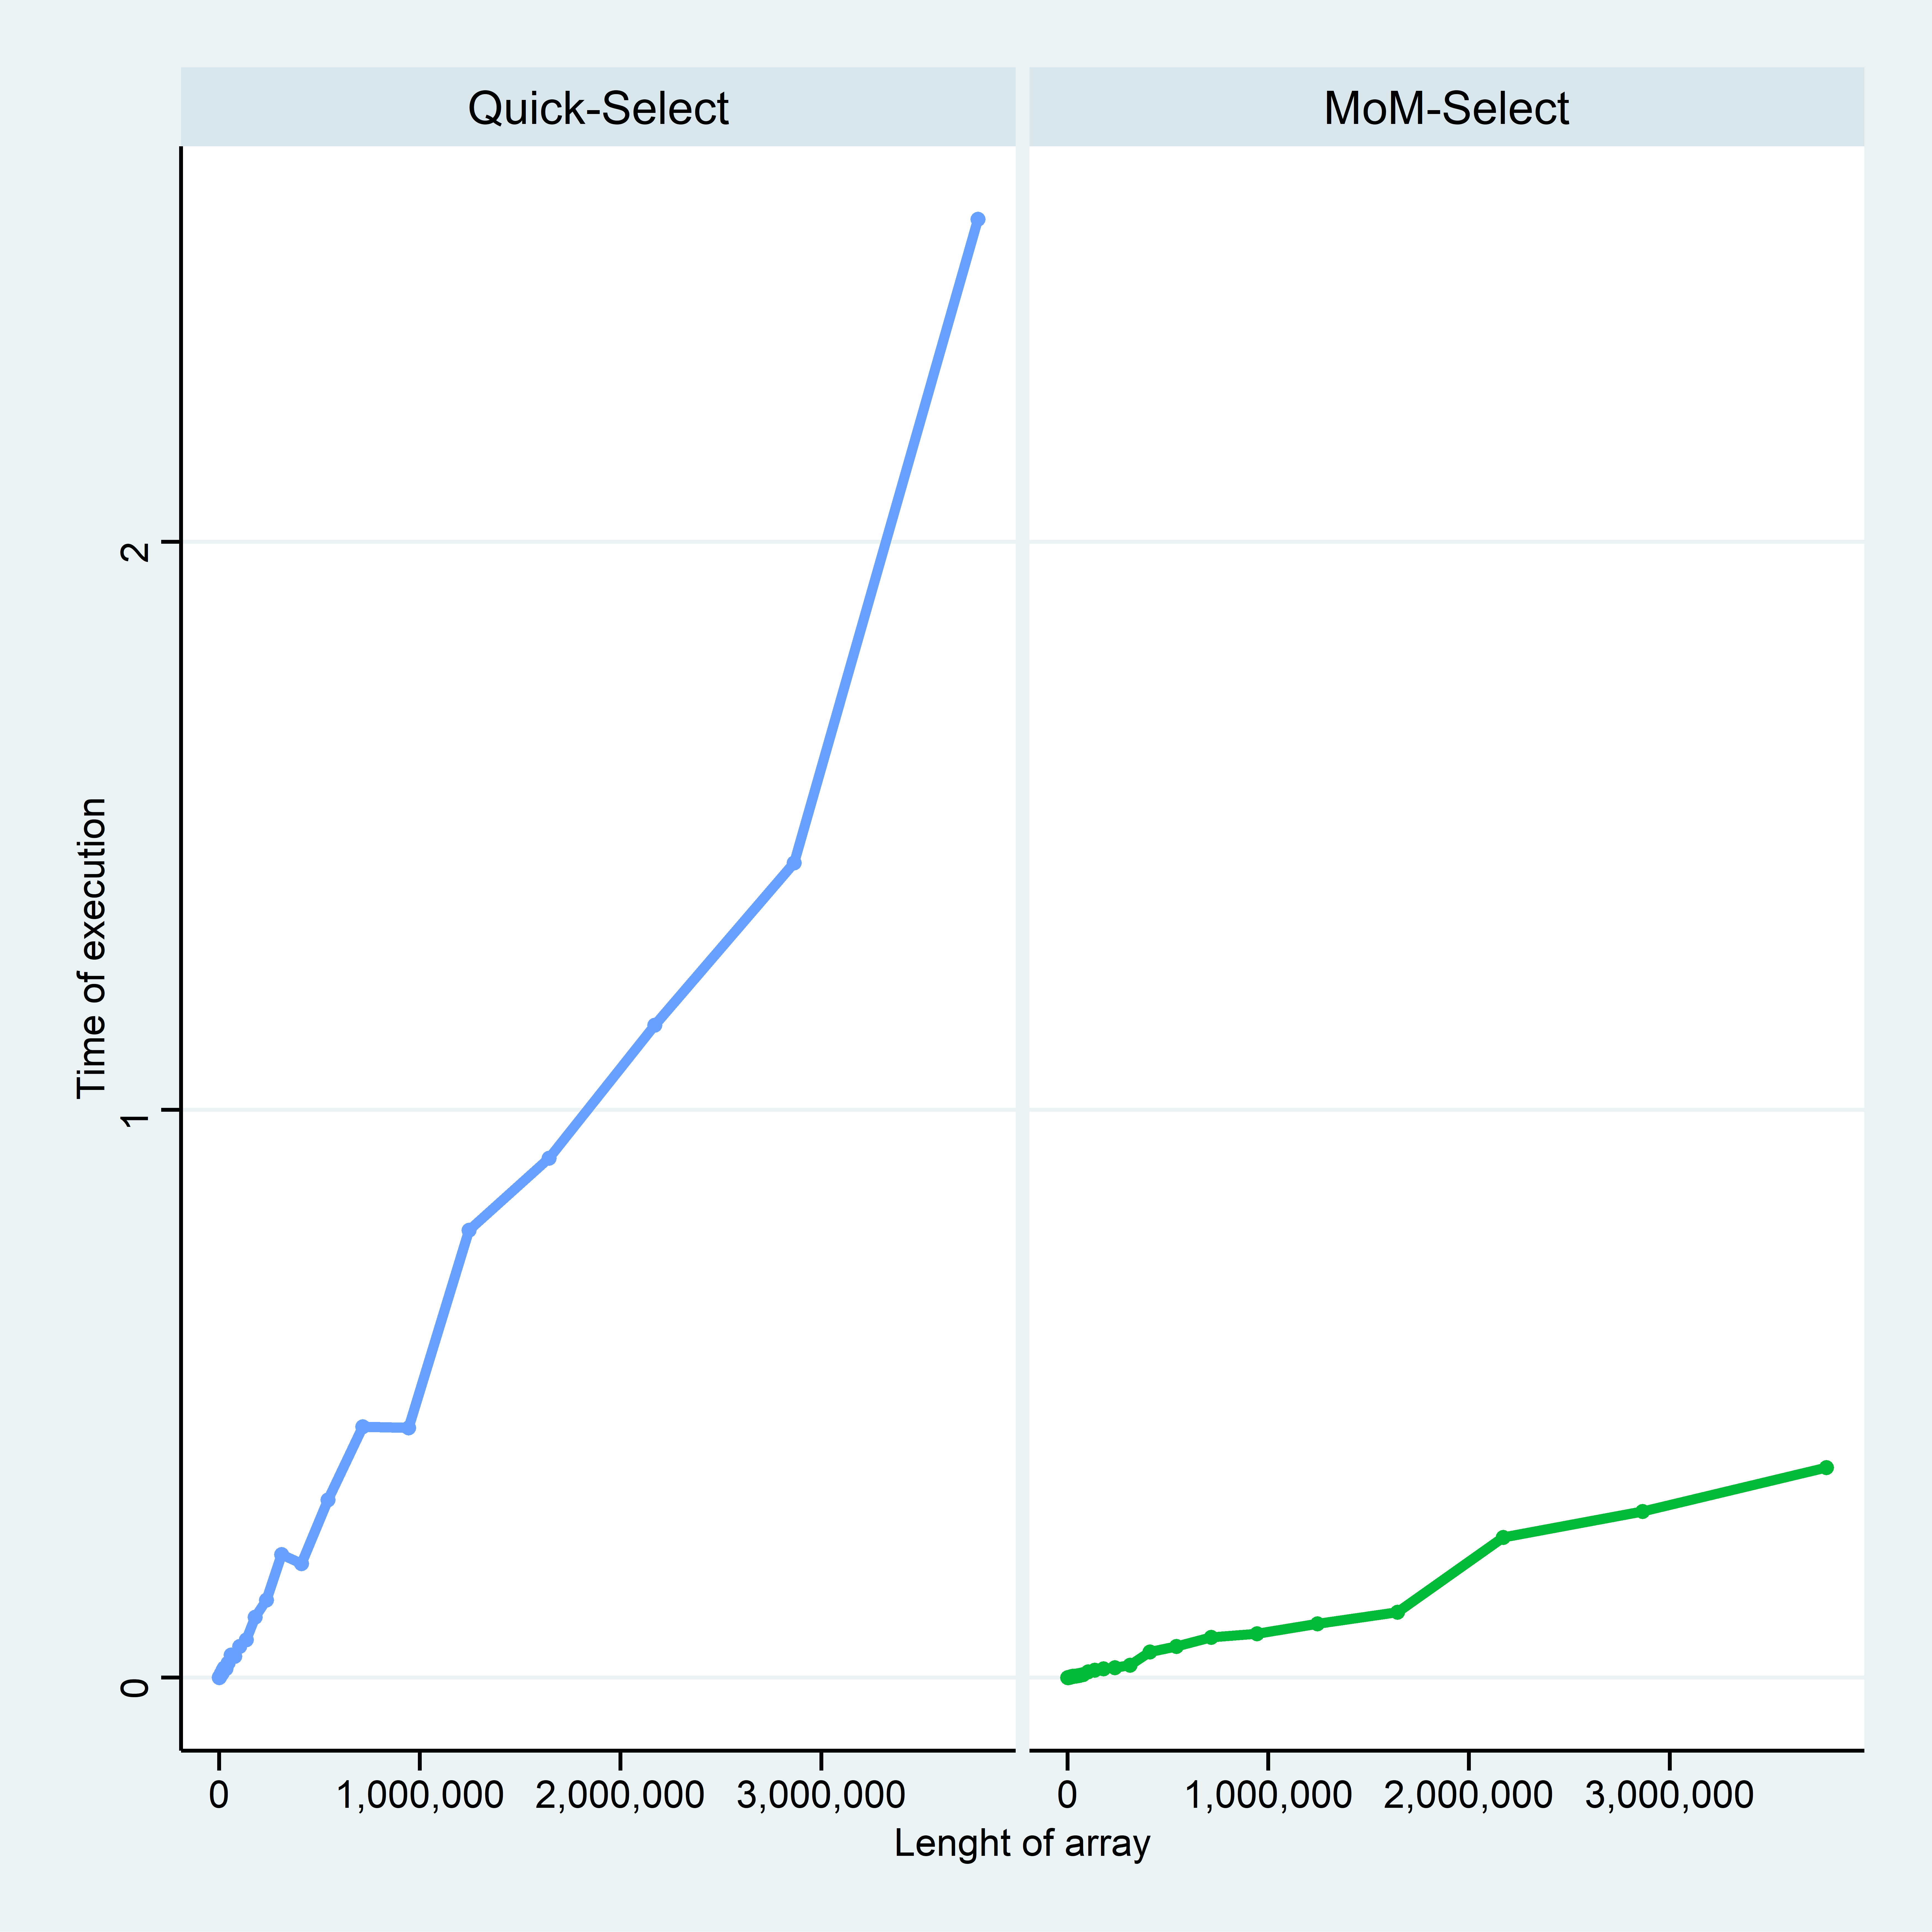
\includegraphics[width=\columnwidth]{images/MoM_Quick_graph_ordered_k1.png}
  		\caption{Tempo di esecuzione a confronto per $n$ variabile e $k=1$ per un array molto ordinato}
  		\label{fig:graph2}
	\end{figure}
	
	Si può inoltre notare una maggiore deviazione mediana assoluta per l'algoritmo QuickSelect rispetto a MedianSelect. Questo è giustificato dal fatto che l'algoritmo MedianSelect, scegliendo sempre un buon perno, compie una quantità di lavoro sempre simile, mentre QuickSelect è più variabile data la scelta del perno casuale che potrebbe, o meno, portare a chiamate ricorsive sbilanciate.
	\\\\
	A fronte di queste considerazioni, il grafico del tempo di esecuzione di HeapSelect risulta in linea con le ipotesi teoriche formulate precedentemente. Questo infatti è denotato da una non linearità giustificata dalla scelta di $k=\frac{n}{3}$. 
	\\
	Si può inoltre notare come la deviazione mediana assoluta sia minore per HeapSelect rispetto a quella degli altri due algoritmi. Ciò è giustificato dal funzionamento della procedura stessa: dato che il numero di operazioni di $extract$ eseguite da HeapSelect è, per $k$ fissato, sempre uguale, risulta ragionevole che complessivamente il costo dell'algoritmo in diverse esecuzioni sia molto simile. 
		
	\newpage
	
	\subsection{Lunghezza $n=75000$ e $k$ variabile in $[0,n-1]$}
	Dato che il tempo di esecuzione dell'algoritmo HeapSelect è dipendente da $k$ mentre quello di QuickSelect e MedianSelect non dovrebbe esserlo, analizziamo il comportamento degli algoritmi al variare di questo parametro.
	
	\begin{figure}[h!]
  		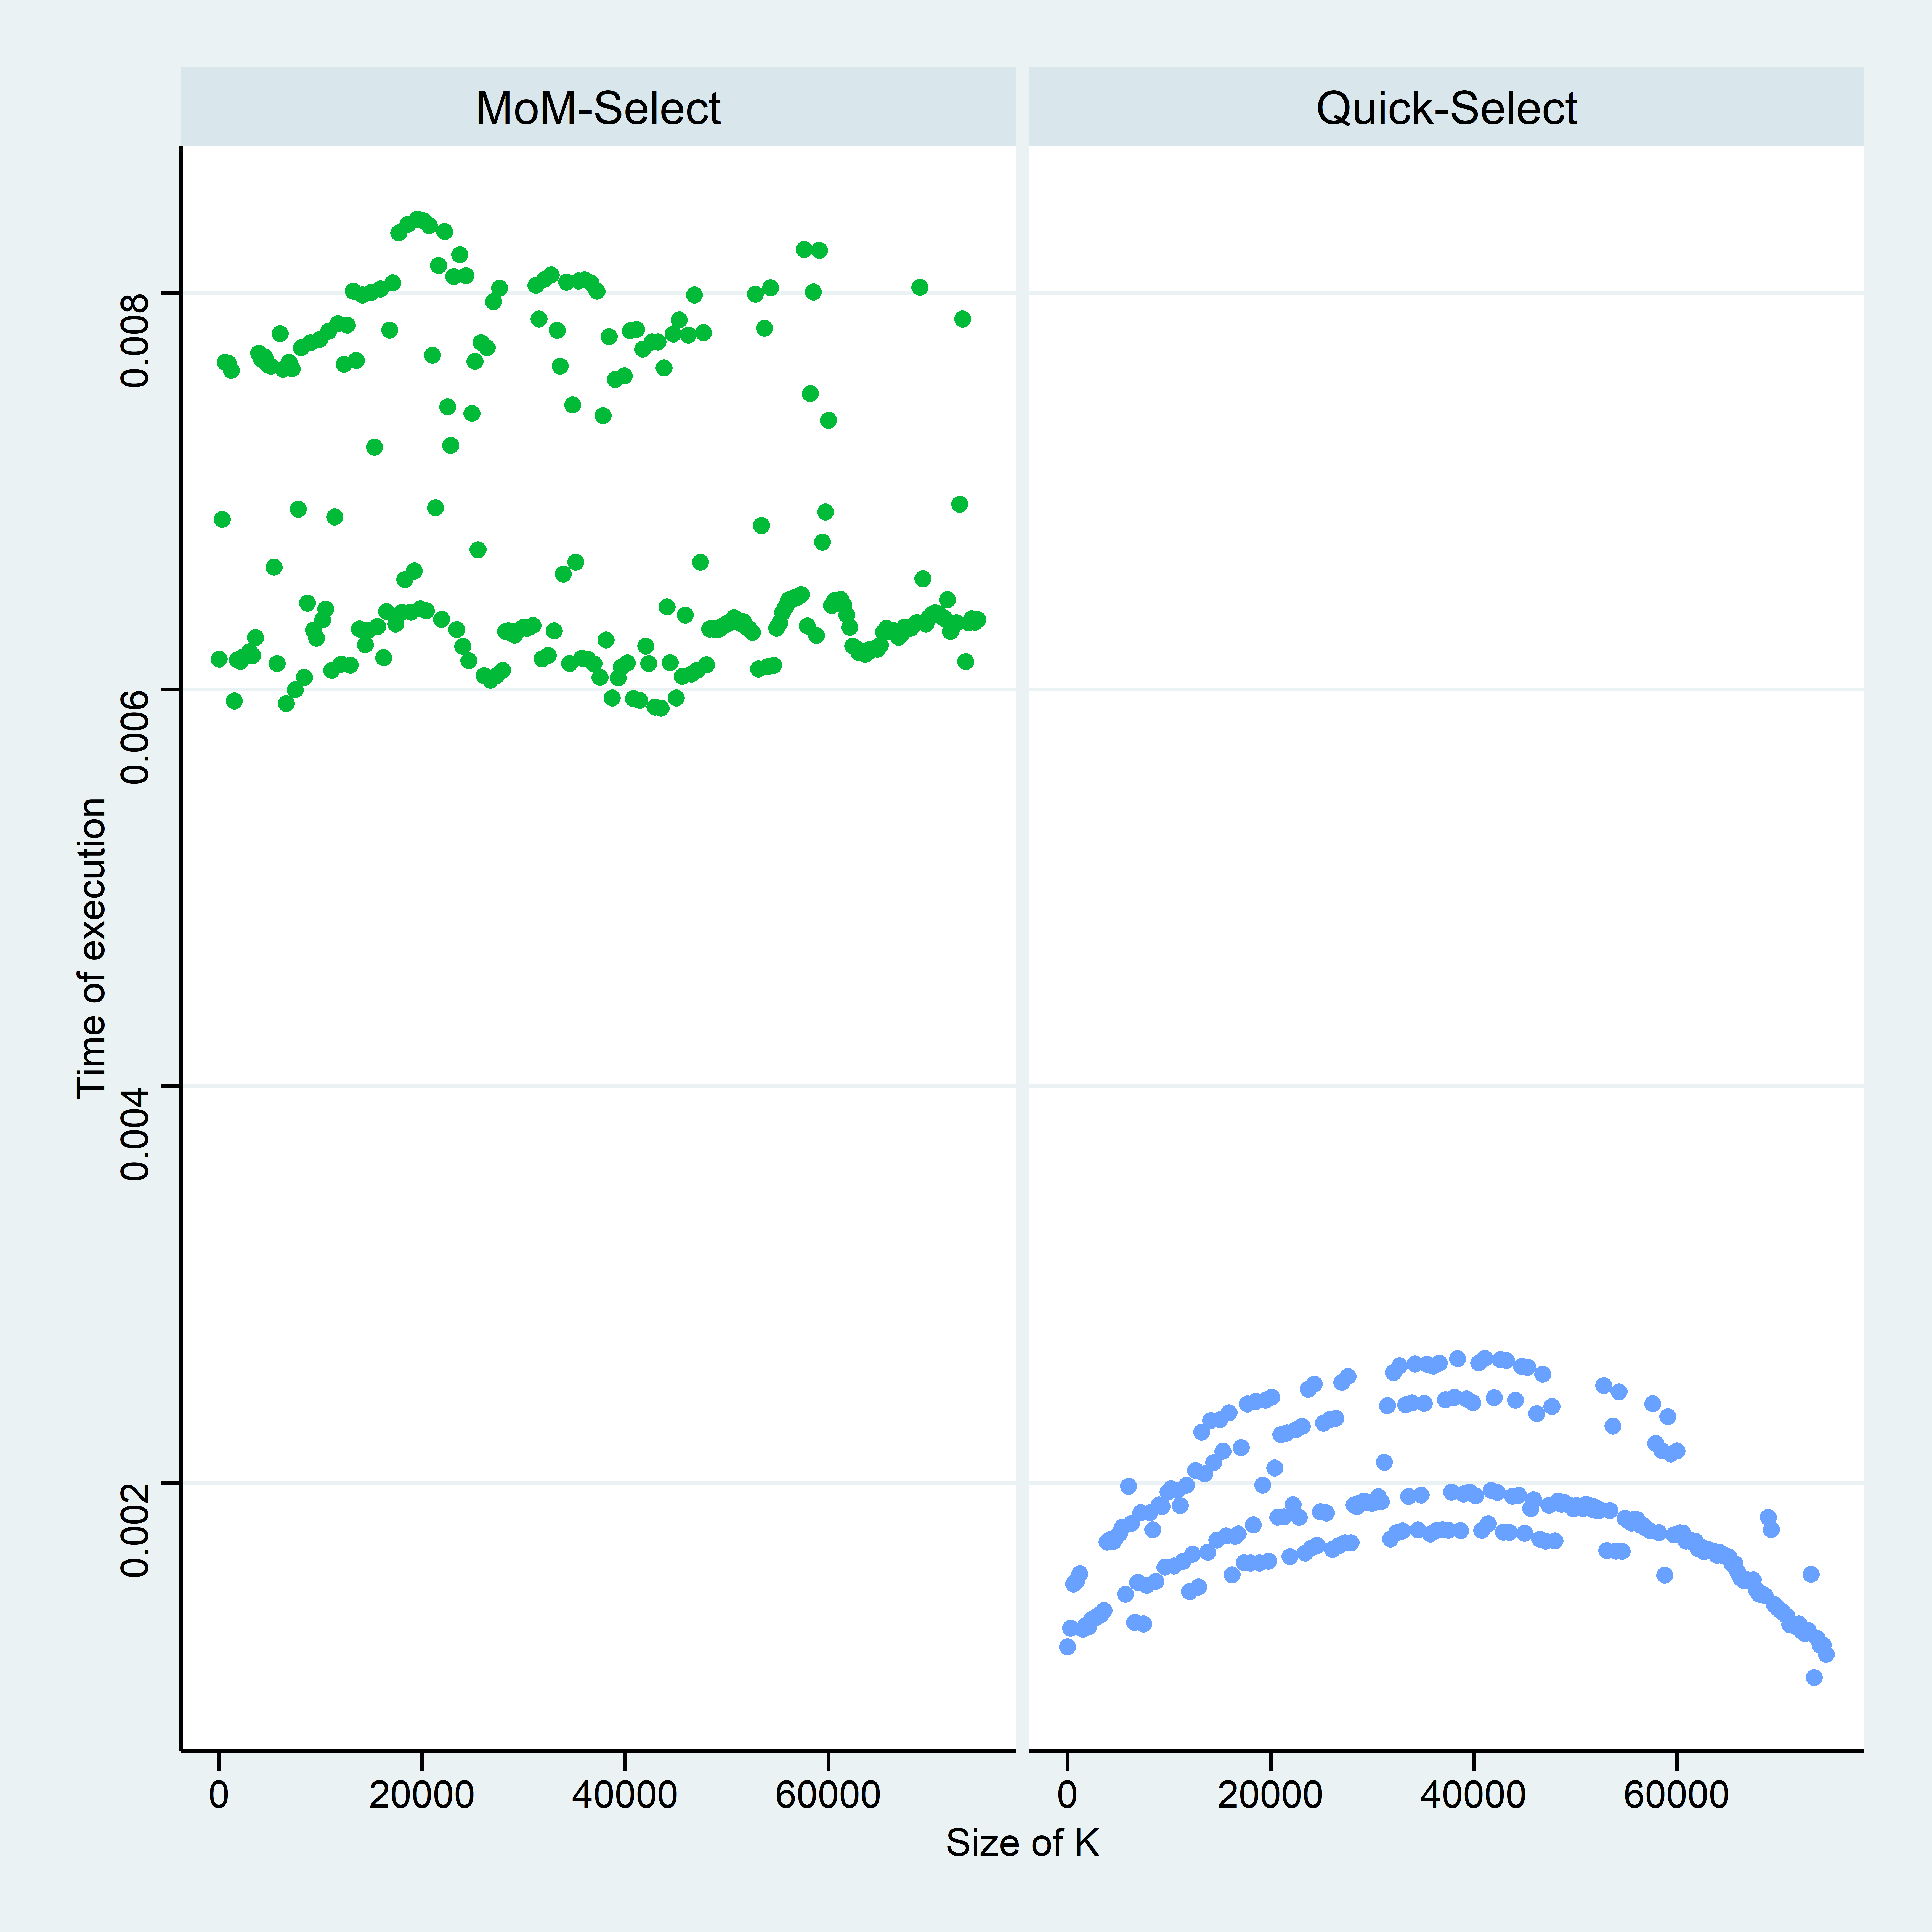
\includegraphics[width=\linewidth]{images/MoM_Quick_graph.png}
  		\caption{Tempo di esecuzione di QuickSelect e MedianSelect per $n=75000$ e $k$ variabile}
  		\label{fig:graph3}
	\end{figure}
	
	Dal grafico si può subito notare come gli algoritmi QuickSelect e MedianSelect non siano effettivamente influenzati dal parametro che stiamo considerando. Questo era prevedibile, dato che il costo asintotico degli algoritmi non è influenzato dal parametro $k$. Questi due algoritmi impiegano infatti tempo pressocchè lineare anche al variare di $k$.
	\newpage
	
	\begin{figure}[h!]
  		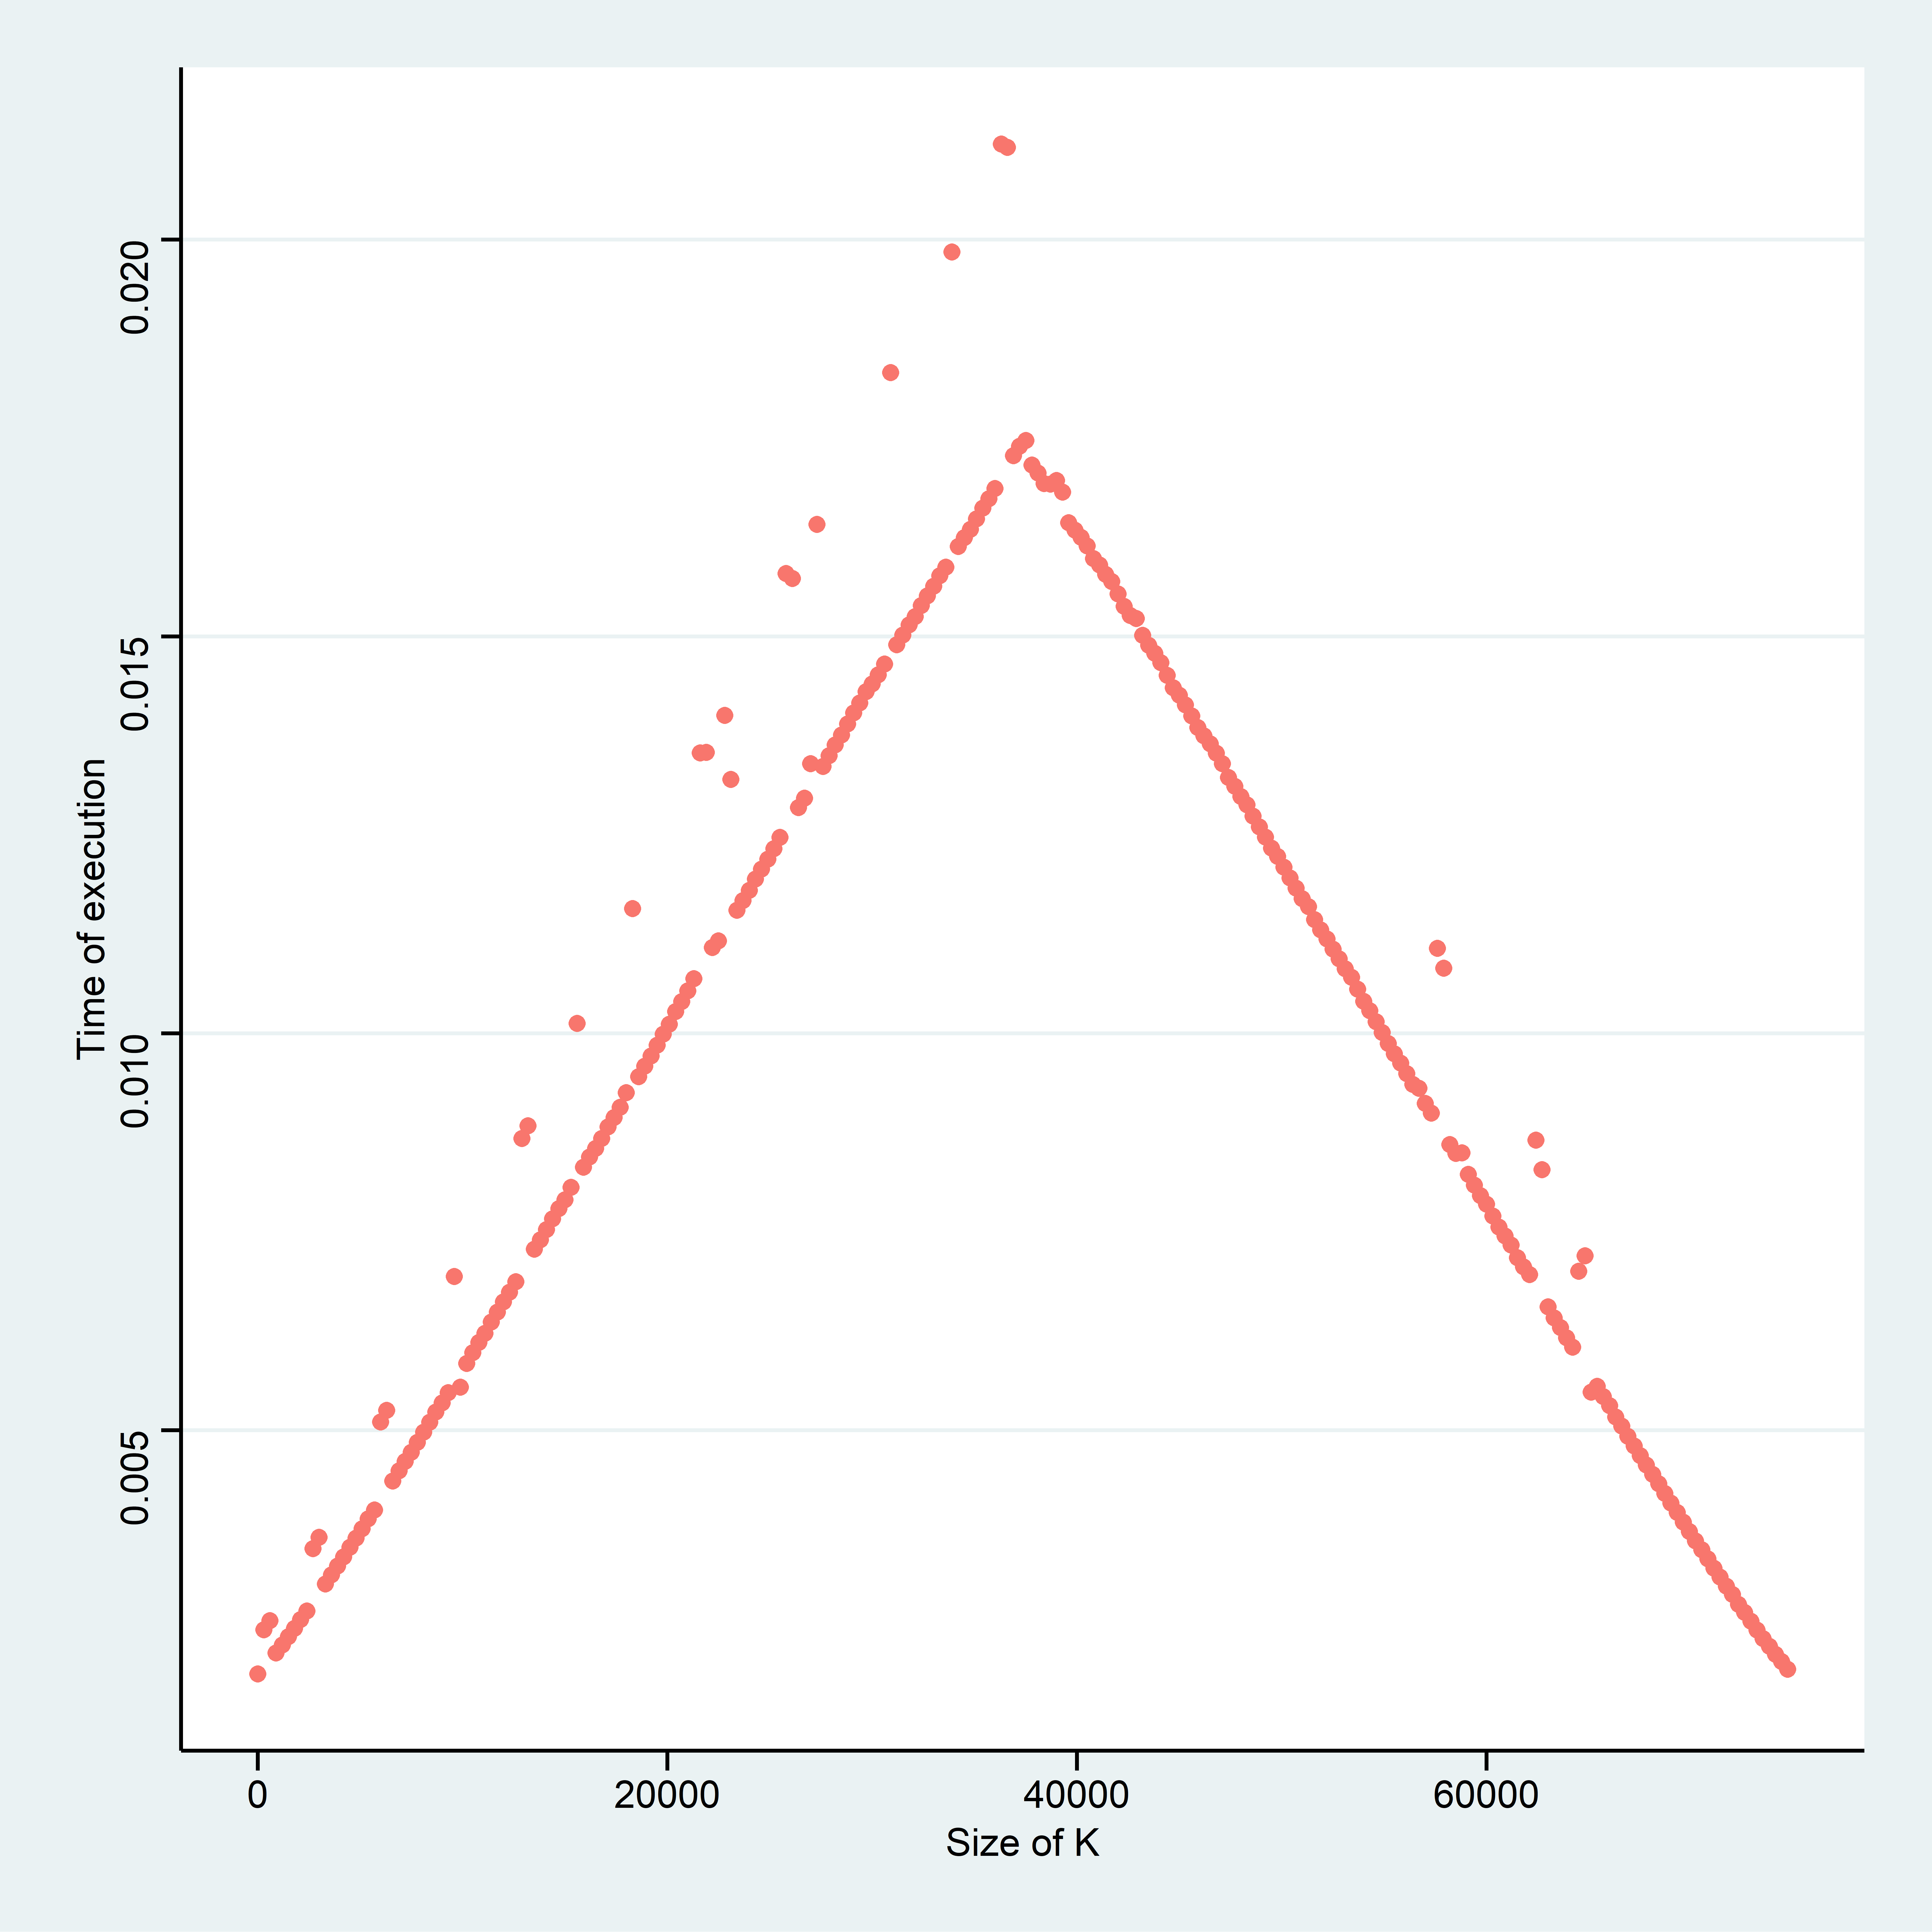
\includegraphics[width=\linewidth]{images/HeapSelect_Kvariable.png}
  		\caption{Tempo di esecuzione di HeapSelect per $n=75000$ e $k$ variabile}
  		\label{fig:graph4}
	\end{figure}
	
	Il caso più interessante è quello di HeapSelect. Il suo costo è effettivamente influenzato da $k$ e questo lo si può notare anche nei tempi sperimentali ottenuti. In particolare, il grafico conferma quanto si era ipotizzato in precedenza nelle Note Implementative (sezione \ref{section:impl_notes}). 
	\\
	Il tempo di esecuzione dell'algoritmo cresce fino a $\frac{n}{2}$, per poi tornare a discendere. Questo è in linea con l'equazione \eqref{eq:heap} che riporta il costo modificato di HeapSelect.
	
	
	\newpage
	Si può osservare anche questo plot 3D in cui variano sia $n$ che $k$. La forma complessiva del grafico è in linea con quanto osservato finora. 
	
	\begin{figure}[h!]
		\centering
		\animategraphics[height=0.8\linewidth, autoplay, loop]{12}{images/gif/heap3d-}{0}{121}
  		\caption{Tempo di esecuzione di HeapSelect per $n$ e $k$ variabili}
  		\label{fig:graph5}
	\end{figure}
		
	\newpage
	
	
	\subsection{Lunghezza $n$ variabile e $k=1$}
	L'ultimo caso di interesse è quello in cui il parametro $k$ è fissato a $1$. Questo caso è interessante in quanto l'algoritmo HeapSelect, essendo influenzato dal parametro $k$, dovrebbe risultare molto più efficiente rispetto al caso generale, impiegando tempo $\Theta\left(n\right)$.
	
	\begin{figure}[h!]
  		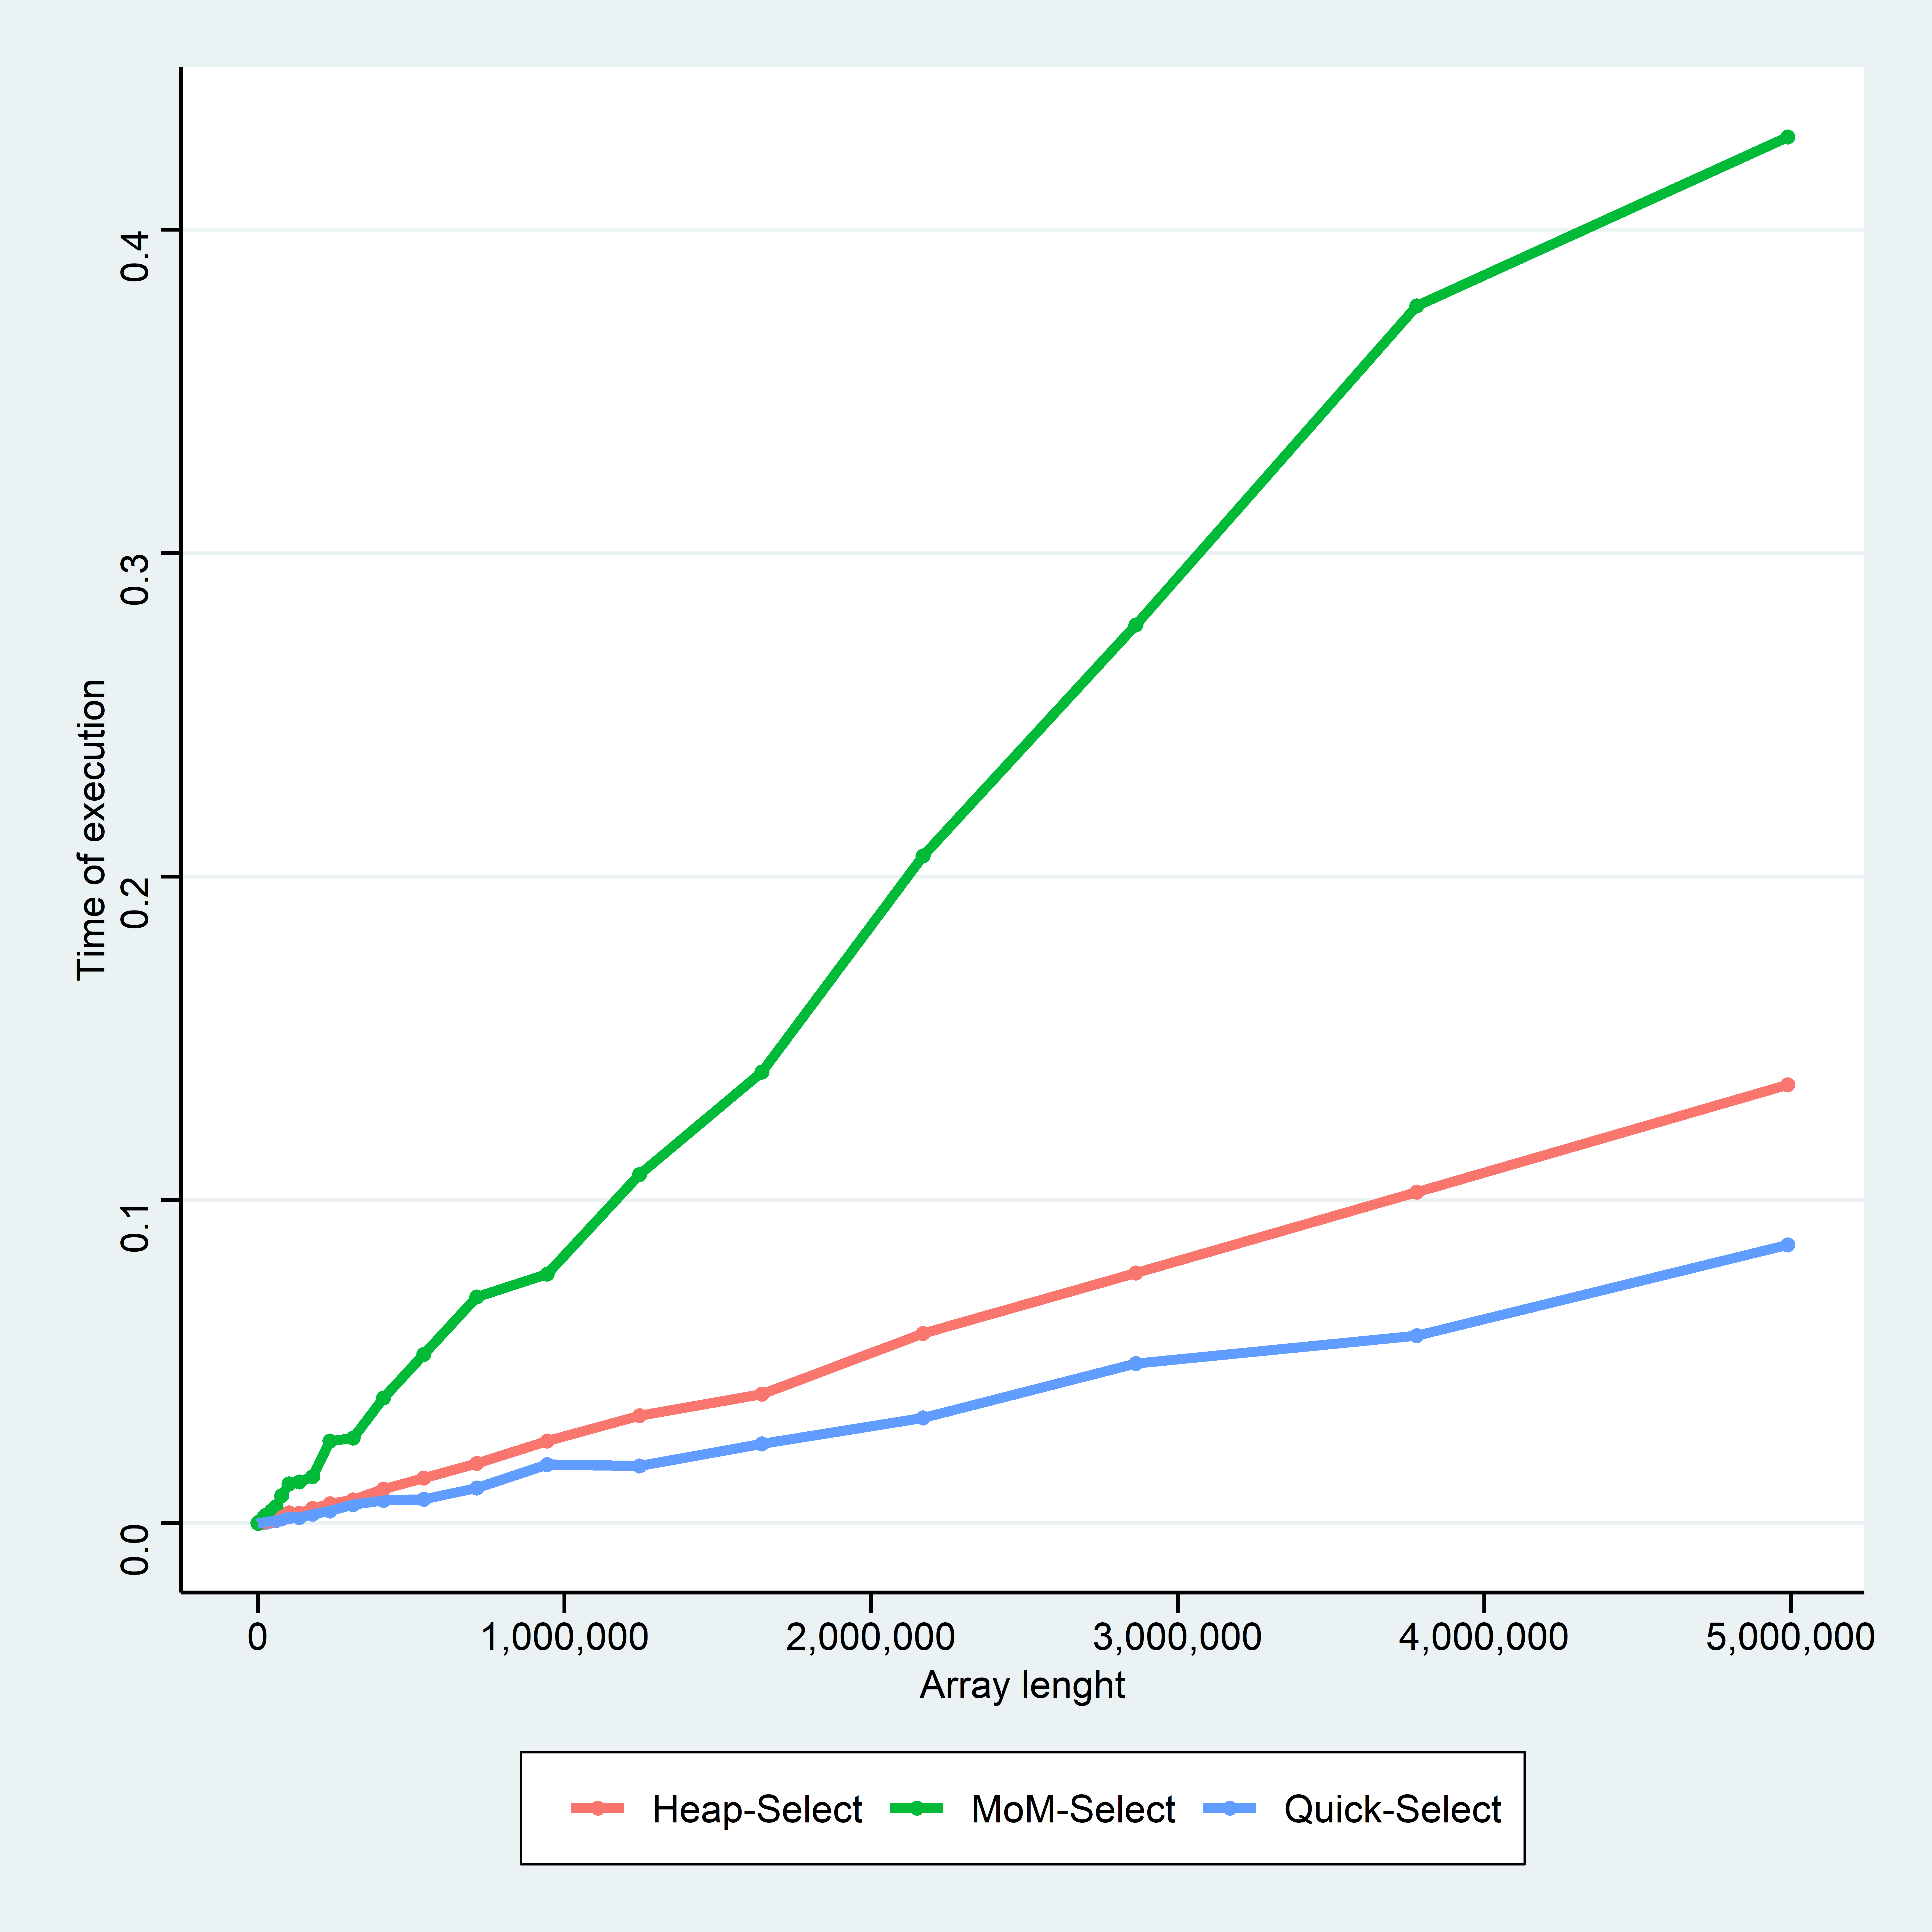
\includegraphics[width=\linewidth]{images/Grafico_Con_K1.png}
  		\caption{Tempo di esecuzione per $n$ variabile a $k=1$}
  		\label{fig:graph6}
	\end{figure}
	
	Dal grafico si può notare come le aspettative teoriche siano effettivamente state rispettate. QuickSelect continua ad essere l'algoritmo più efficiente per gli stessi motivi di cui sopra (sezione \ref{subsection:nvar_k_n3}), ma ora HeapSelect risulta più efficiente di MedianSelect in quanto deve effettuare una quantità di lavoro sempre lineare (e minore di quella che compie MedianSelect per la scelta di un buon perno e le successive chiamate ricorsive).
		
	\newpage

	\begin{figure}[h!]
  		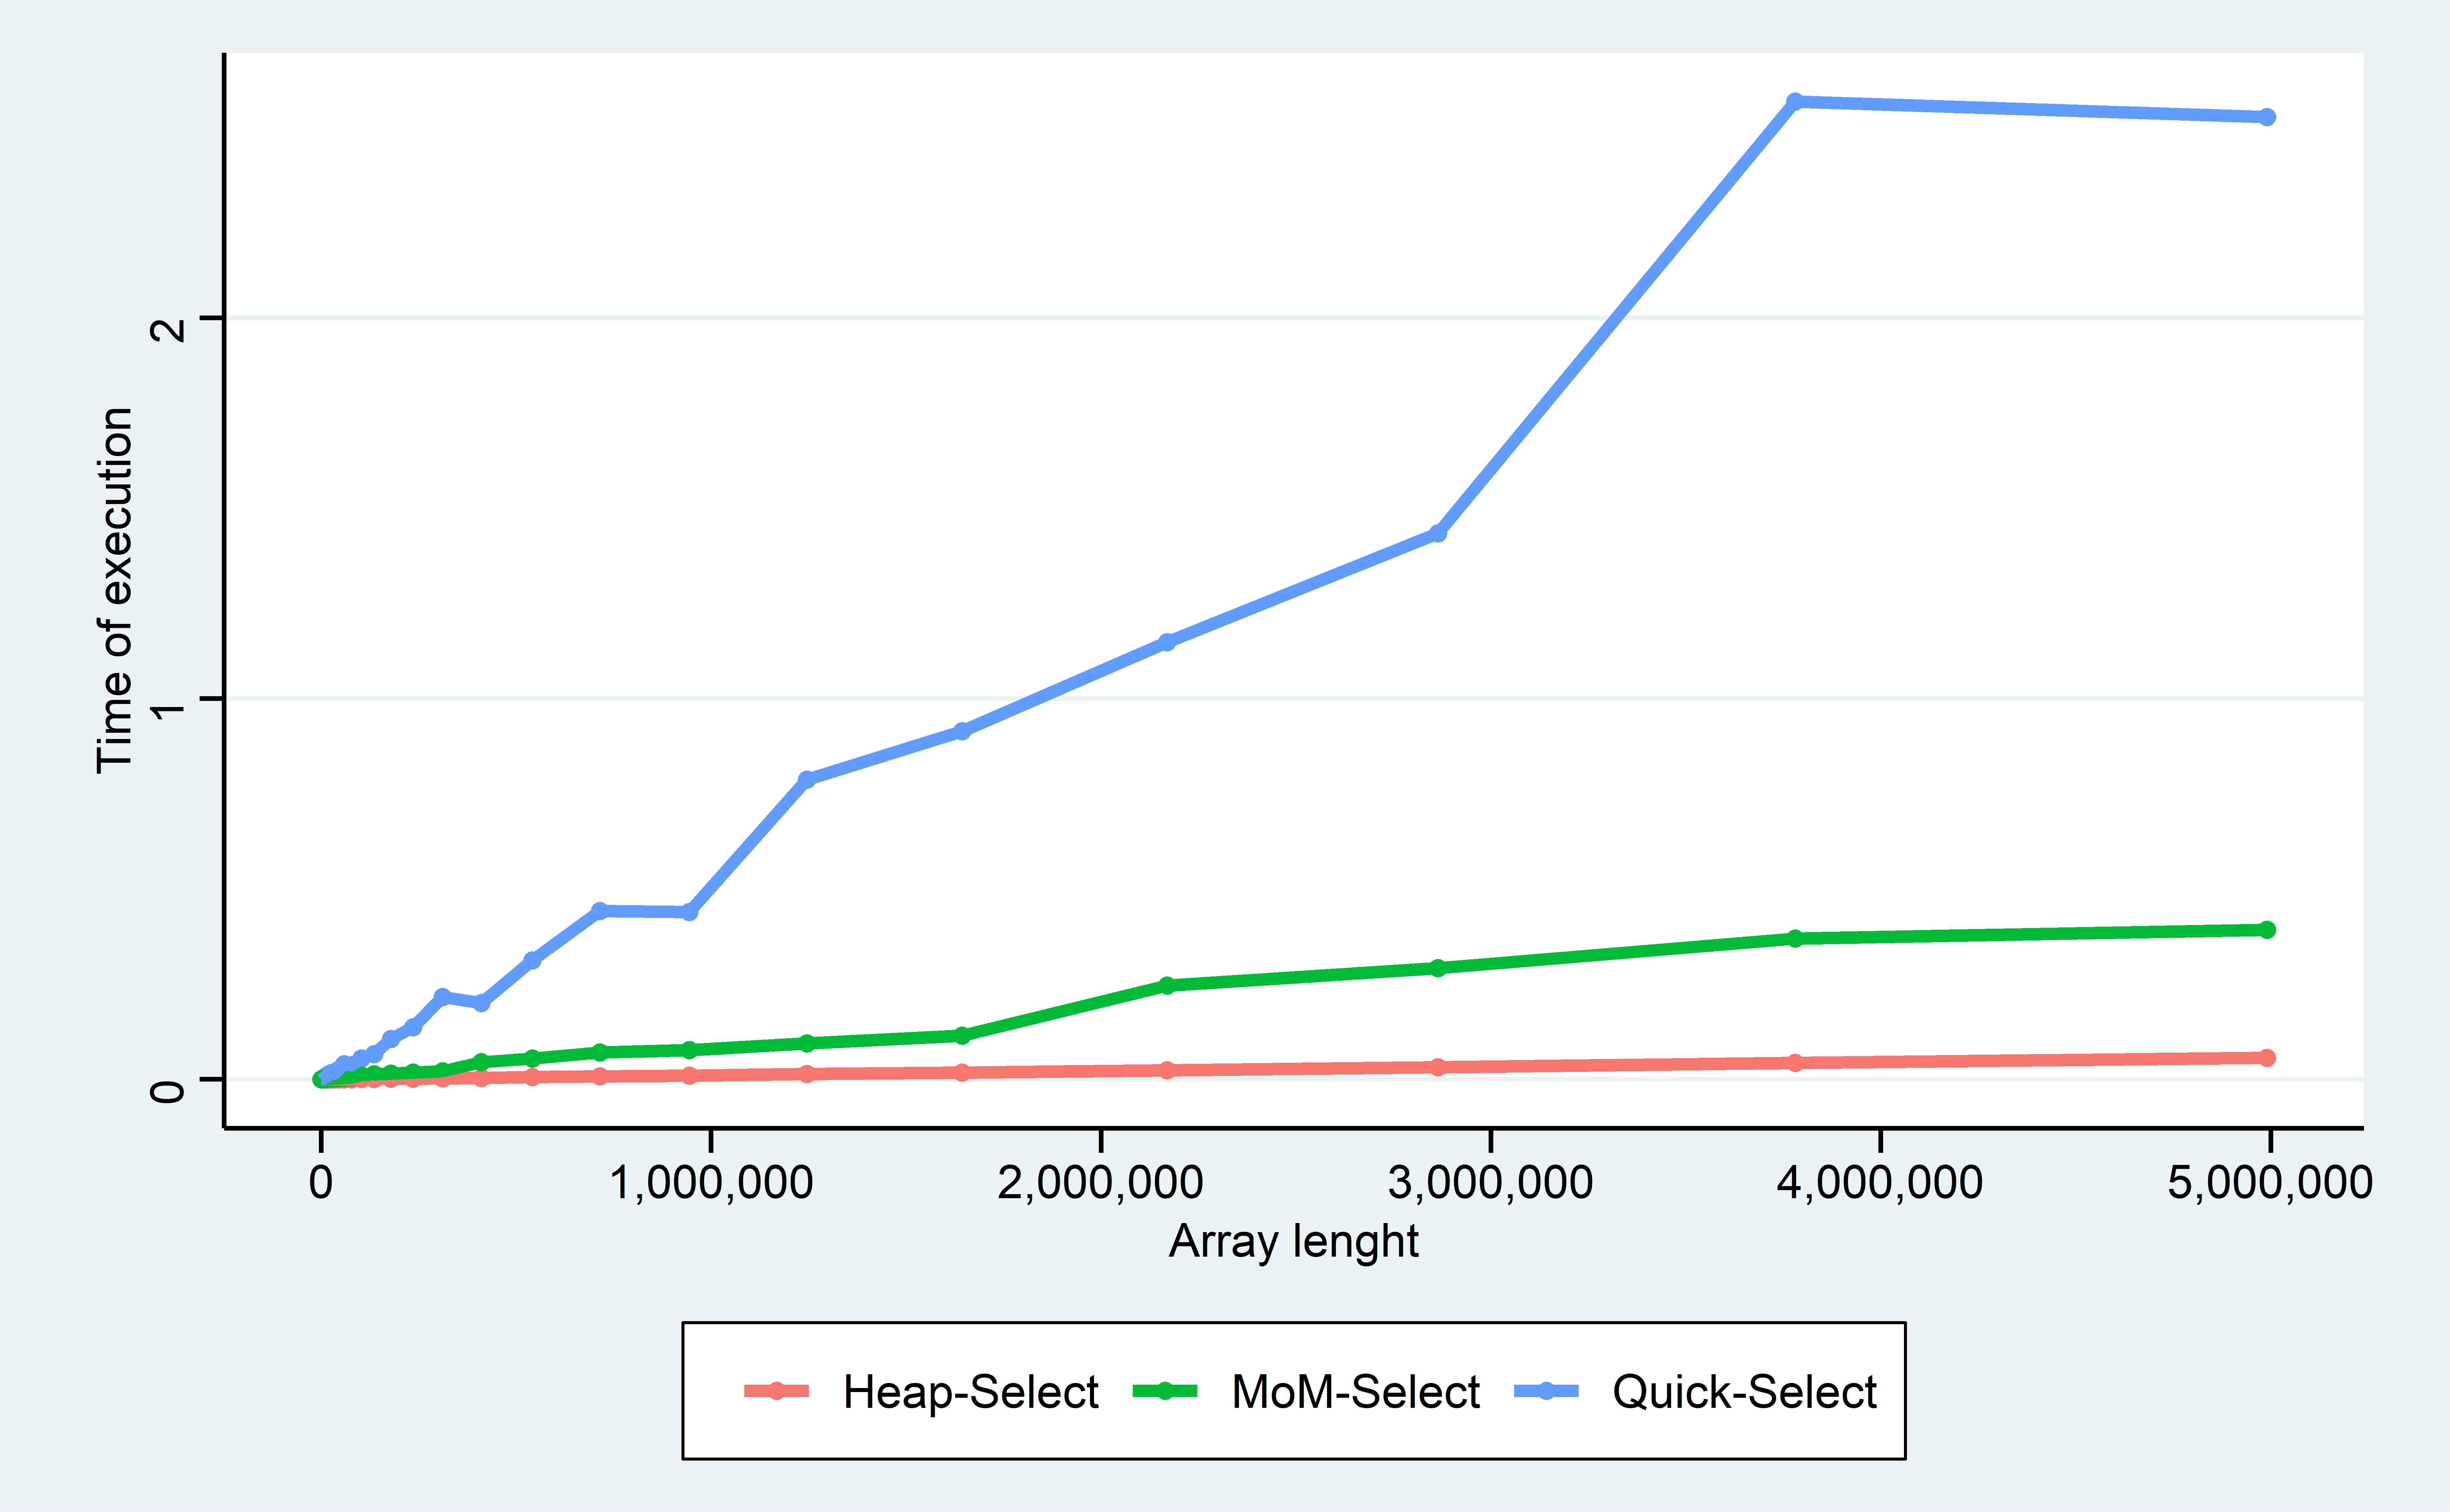
\includegraphics[width=\linewidth]{images/All_graph_ordered_k1.png}
  		\caption{Tempo di esecuzione per $n$ variabile a $k=1$ per un array molto ordinato}
  		\label{fig:graph6}
	\end{figure}
	Come si può notare, HeapSelect risulta l'algoritmo più efficiente, fra quelli in analisi, nel caso di array di input fortemente ordinati e $k=1$. Ciò è in linea con le aspettative teoriche enunciate nella sezione \ref{section:theory}.
	
	\newpage

	\section{Conclusioni}
	I risultati ottenuti sono stati molto interessanti e, a tratti, inaspettati. L'analisi sperimentale degli algoritmi in questione ha certamente contribuito ad una maggior consapevolezza nell'uso degli stessi.
	\\
	Si può trarre la seguente conclusione dall'analisi sperimentale effettuata sugli algoritmi: ogni algoritmo ha dei punti di forza e di debolezza. In particolare, QuickSort risulta sempre il più efficiente per array di input casuali, HeapSelect risulta il più stabile e anche molto efficiente per $k\approx 1 $ o $k \approx n$, mentre MedianSelect si conferma essere un algoritmo ottimo per qualsiasi array di input.
	
\end{document}
